\subsection{Unsicherheiten} \label{subsec:MRCPSP_Unsicherheiten}

Insbesondere in der Realität ist es möglich, dass Unsicherheiten auftreten können. Dies kann der Fall sein, wenn Events, wie der Ausfall von Maschinen, die Erkrankung von Mitarbeitern, die Fehleinschätzung bei der Planung usw. auftreten \cite[vgl.][S. 64 ff.]{deblaere_reactive_2011}. Durch Verspätungen können Projekte in Verzug kommen und somit die geplante Makespan $C_{max}$ überschreiten. Dies ist suboptimal und stellt eine Herausforderung bei der Erzeugung von Zeitplänen dar. Mit solchen Unsicherheiten gilt es auf abstrakter Ebene innerhalb des (M)RCPSP umzugehen. \\

Es können verschiedene Arten von Unsicherheiten betrachtet werden. Die in der Literatur am häufigsten aufzufindenden Unsicherheitsarten sind Verspätungen von Aktivitäten und erneuerbaren Ressourcen, die nicht zu jedem Zeitpunkt konstant vorliegen. \cite[vgl.][S. 64 ff.]{deblaere_reactive_2011} \\

Störungen der Aktivitätsdauer treten auf, wenn die tatsächliche Dauer einer Aktivität größer ist, als die geplante Dauer $d_j$. Die Differenz zwischen geplanter und tatsächlicher Dauer wird über $\Delta_j \in \mathbb{N}$ ausgedrückt. \cite[vgl.][S. 65]{deblaere_reactive_2011} Dies wird in Abbildung \ref{img:example_mrcpsp_schedule_activitydisturbance} anhand des MRCPSP Beispiel-Zeitplans aus Abschnitt \ref{subsec:MRCPSP_MM} bei der Aktivität 4 mit $\Delta_4$ = 1 deutlich. Zudem lässt sich erkennen, dass der geplante Makespan gegenüber dem initialen Zeitplan (Abbildung \ref{img:example_mrcpsp_schedule}) trotz der Störung nicht in Vorzug kommt, da die Verspätung über den Puffer von einer Zeiteinheit und einer verfügbaren Ressource $R_1$ und mehreren Ressourcen $R_2$ vor Durchlauf der Folgeaktivität bedient werden konnte. 

\begin{figure}[H]
    \centering
    \noindent\makebox[\textwidth]{%
    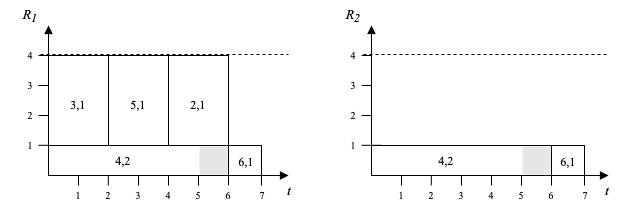
\includegraphics[width=1\textwidth]{assets/img/02_Grundlagen/ExampleProjectMRCPSP_ScheduleDelay.drawio.png}
    }
    \caption{MRCPSP Beispiel-Zeitplan mit einer Aktivitätsstörung von $\Delta_4$ = 1} 
    \label{img:example_mrcpsp_schedule_activitydisturbance}
    \source{Eigene Darstellung}
\end{figure}

Eine weitere Art von Unsicherheiten stellen Störungen bei den erneuerbaren Ressourcen dar. Bei dieser Störungsart besteht die Annahme, dass die Anzahl der verfügbaren Ressourcen einer Ressourcenart $R_k$ zu einem Zeitpunkt $t$ über die Differenz $\Delta^\rho_k \in \mathbb{N}$ reduziert wird. Über $t + \delta_t$ wird angegeben, ab welchem Zeitpunkt die erneuerbaren Ressourcenarten wieder komplett zur Verfügung stehen \cite[vgl.][S. 65 f.]{deblaere_reactive_2011}. Abbildung \ref{img:example_mrcpsp_schedule_resourcedisturbance} verdeutlicht die erneuerbaren Ressourcenstörungen. Im Zeitintervall $[4, 7]$ befindet sich eine erneuerbare Ressourcenstörung $\Delta^\rho_1 = 1$. Aktivität 2 kann somit nicht planmäßig ab Zeiteinheit 4 gestartet werden, da durch die Störung nicht genügend erneuerbare Ressourcen für den ausgewählten Modus vorhanden sind. Somit muss entweder ein anderer Modus ausgewählt werden oder solange mit dem Start von Aktivität 2 gewartet werden, bis die erneuerbaren Ressourcen für die komplette Laufzeit der Aktivität wieder zur Verfügung stehen. Der Start der Ausführung wäre bei dem selektierten Modus ab $t = 5$ der Fall, da durch das Fertigstellen von Aktivität 4 eine erneuerbare Ressource $R_1$ freigegeben wird und somit die erforderliche Anzahl von Ressourcen ($r_{2,1,1} = 3$) zur Verfügung stehen. Dadurch kommt jedoch bei Aktivität 6 ein Startverzug von einer Zeiteinheit. Durch diese Störung erhöht sich der Makespan des Zeitplans aus Abbildung \ref{img:example_mrcpsp_schedule_resourcedisturbance} ($C_{max} = 8$) gegenüber dem Zeitplan aus Abbildung \ref{img:example_mrcpsp_schedule} ($C_{max} = 7$) um eine Zeiteinheit.

\begin{figure}[H]
    \centering
    \noindent\makebox[\textwidth]{%
    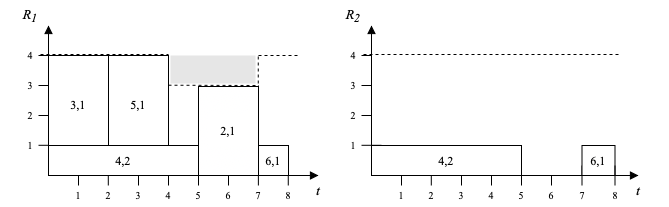
\includegraphics[width=1\textwidth]{assets/img/02_Grundlagen/ExampleProjectMRCPSP_ScheduleResourceDelay.drawio.png}
    }
    \caption{MRCPSP Beispiel-Zeitplan mit einer (erneuerbaren) Ressourcenstörung ab $t$ = 4 von $\Delta_1^\rho$ = 1, welche ab $t + \delta_t = 7$ normalisiert wird} 
    \label{img:example_mrcpsp_schedule_resourcedisturbance}
    \source{Eigene Darstellung}
\end{figure}

Das Ziel des (M)RCPSP besteht darin, den Zeitplan mit der geringsten Projektausführungsdauer zu finden. Der Umgang mit Unsicherheiten stellt zudem eine Herausforderung dar. \cite{brcic_resource_2012} beleuchtete in einer Erhebung einige Möglichkeiten zum Umgang des Unsicherheitsproblems für die stochastische Version des RCPSP. \\

Die naivste Herangehensweise mit Unsicherheiten umzugehen ist es diese bei der Zeitplanerstellung zu ignorieren. Diese Methode wird von \cite{brcic_resource_2012} als prädiktiv bezeichnet. Das Ignorieren von Unsicherheiten kann jedoch dazu führen, dass der Zeitplan durch Verspätungen stärker in Verzug kommt als bei anderen Herangehensweisen. \cite[vgl.][S. 404]{brcic_resource_2012} \\

Die proaktive Herangehensweise behandelt das Problem der Unsicherheiten, indem eine weitere Zielfunktion, nämlich die Robustheit eingeführt wird \cite[vgl.][S. 404]{brcic_resource_2012}. Die Robustheit gibt an, dass der Zeitplan mit geringfügigen Veränderungen (z. B. die der Unsicherheitszenarien) von Aktivitäten umgehen kann \cite[vgl.][S. 246]{khemakhem_efficient_2013}. \\

Die dritte Herangehensweise stellt die reaktiven Methoden dar. Diese reagieren direkt zum Zeitpunkt der Unsicherheit. Hierbei besteht die Möglichkeit, den Zeitplan ab der Unsicherheitsstelle zu reparieren oder gänzlich ab der Stelle der Unsicherheit einen neuen Zeitplan zu erstellen \cite[vgl.][S. 404 f.]{brcic_resource_2012}.  \\

In der Literatur werden prädiktive Verfahren auch als proaktive Verfahren bezeichnet und umgekehrt \cite[vgl.][S. 246]{khemakhem_efficient_2013}. Im Rahmen der Masterarbeit werden folglich die eingangs vorgestellten proaktiven Verfahren nun als prädiktive Verfahren behandelt, welche z. B. die Robustheit optimieren. Die eingangs vorgestellten prädiktiven Verfahren werden somit als proaktive Verfahren angesehen, welche z. B. Unsicherheiten ignorieren. Im Abschnitt  \ref{subsec:Praediktive_Methoden} werden die prädiktiven Methoden, repräsentierend durch die Robustheit,s konkreter vorgestellt. Die reaktiven Methoden, repräsentierend durch das Erzeugen von neuen Zeitplänen zu den Unsicherheitszeitpunkten, werden im Abschnitt \ref{subsec:Reaktive_Methoden} vorgestellt.

\subsubsection{Prädiktive Methoden}
\label{subsec:Praediktive_Methoden}

Eine Möglichkeit mit Unsicherheiten umzugehen stellt das vorausschauende Erstellen von Zeitplänen dar. Hierbei wird neben der Minimierung der Projektdauer $C_{max}$ eine weitere Zielfunktion eingeführt, nämlich die Maximierung der Robustheit $\Omega$. Die Robustheit gilt als die Maßeinheit, wie gut mit kleinen Änderungen innerhalb eines Zeitplans umgegangen werden kann, ohne dass die Projektdauer durch die Verspätung ansteigt \cite[vgl.][S. 246]{khemakhem_efficient_2013} \cite[vgl.][S. 177]{al-fawzan_bi-objective_2005}. \\

Eine mögliche Messung von Robustheit kann über die Summe aller freien Puffer der Aktivitäten definiert werden. Unter einem freien Puffer $s_j$ werden die Zeiteinheiten verstanden, die eingesetzt werden können, damit die unmittelbare Folgeaktivität nicht verzögert wird. Die Einhaltung der Ressourcenbeschränkung muss im Puffer dennoch berücksichtigt werden. Folglich ist die Robustheit über $\Omega = \sum_{j=1}^n s_j$ definiert. \cite[vgl.][S. 177]{al-fawzan_bi-objective_2005} \\

Der freie Puffer lässt sich über die frühsten und spätesten Start- bzw. Endzeitpunkte berechnen $s_j = LST_j - EST_j \Leftrightarrow s_j = LFT_j - EFT_j$. Während $EST_j$ und $EFT_j$ sich über den erstellten Zeitplan ablesen lassen, müssen $LST_j$ und $LFT_j$ über die Backward Recursive Prodecure berechnet werden \cite[vgl.][S. 181]{al-fawzan_bi-objective_2005}. \\

Bei dem \ac{rcpsp} Beispiel-Zeitplan $S^1$ aus Abbildung \ref{img:example_rcpsp_schedule} liegt die Robustheit bei $\Omega^1 = \sum_{j=1}^n s_j = 1$, da der einzige freie Puffer bei Aktivität $j_1$ liegt. Bei einer Verspätung von $\Delta_1 = 1$ würde es zu keiner Verspätung der Projektdauer $C_{max}$ kommen, da der Puffer genutzt werden kann. Sofern es bei einer anderen Aktivität zu einer Verspätung kommt, wird sich die Projektdauer $C_{max}$ verzögern. Ähnlich sieht es bei dem \ac{mrcpsp} Beispiel-Zeitplan $S^2$ aus Abbildung \ref{img:example_mrcpsp_schedule} aus, welcher ebenfalls einen Wert von $\Omega^2 = \sum_{j=1}^n s_j = s_4 = 1$ aufweist. Bei Nutzung des Puffers liegt nach dem Verspätungsszenario $\Delta_4 = 1$ die Robustheit bei $\Omega^{2'} = 0$ (vgl. Abbildung \ref{img:example_mrcpsp_schedule_activitydisturbance}). \\

Ein Zeitplan mit der gleichen Projektdauer $C_{max}$ kann unterschiedliche Robustheitswerte aufweisen und ist folglich für Unsicherheitsszenarien mehr oder weniger geeignet \cite[vgl.][S. 178]{al-fawzan_bi-objective_2005}. Beim prädiktiven Ansatz gilt es bei Zeitplänen mit identischer Projektdauer den mit dem höchsten Robustheitswert auszuwählen. \\

Die Robustheit lässt sich nicht nur über die Summe aller freien Puffer eines Zeitplans definieren. \cite{khemakhem_efficient_2013} vergleicht in seiner Publikation eine Menge von Robustmessungsfunktionen für das RCPSP und stellt das Prinzip der weighted slack functions (dt. gewichtete Pufferfunktionen) vor. Die Slack Function (dt. Pufferfunktion) stellt zum Beispiel die Summe der freien Puffer oder auch einen binärer Puffer dar \cite[vgl.][S. 253 f.]{khemakhem_efficient_2013}. Der Puffer kann anschließend über ein Weight (dt. Gewicht) multipliziert wird. Folglich wirkt sich ein Puffer für dominierende Aktivitäten stärker gegenüber einfachen Aktivitäten aus. Ein Weight kann die Anzahl von notwendigen Ressourcen, direkten oder totalen Nachfolgern einer Aktivität uvw. darstellen \cite[vgl.][S. 254 ff.]{khemakhem_efficient_2013}. Das Kombinieren von mehreren Weights ist ebenfalls möglich \cite[vgl.][S. 254 ff.]{khemakhem_efficient_2013}. \\

Tabelle \ref{tab:SlackFunctions} beinhaltet einen Ausschnitt von Slack Functions, welche von \cite{khemakhem_efficient_2013} vorgestellt wurden. Die Slack Functions können über die ebenfalls von \cite{khemakhem_efficient_2013} vorgestellten Weights aus Tabelle \ref{tab:Weights} gewichtet werden. \\

\begin{table}[H]
\centering
\resizebox{\textwidth}{!}{%
\begin{tabular}{r|l|l}
Slack Function & Beschreibung & Definition \\ \hline
$SF1$ & Summe von freien Puffern & $\sum_{j=1}^n s_j$ \\ \hline
$SF2$ & Summe von binären Puffern & $\sum_{j=1}^n \alpha$ mit $\alpha = \left\{\begin{array}{ll} 
        1 & \text{wenn $s_j > 0$} \\
        0 & \text{sonst} \\
     \end{array}\right. $ \\ \hline
$SF3$ & \begin{tabular}[c]{@{}l@{}}Minimum zwischen freien Puffer und \\ Bruchteil der Aktivitätsdauer $d_j$\end{tabular} &          $\sum_{j=1}^n \min (s_j, frac * d_j) $ mit $frac \in (0, 1) $  \\ \hline
$SF4$ & Funktion zum Verringern des freien Puffers & $\sum_{i=1}^{s_j} e^{-i}$ \\ \hline
... & ... & ...       
\end{tabular}
}%

\caption{Definitionen von Slack Functions zur Robustheitsmessung}
\label{tab:SlackFunctions}
\source{In Anlehnung an \cite[S. 254]{khemakhem_efficient_2013}}
\end{table}

\begin{table}[H]
\centering
\resizebox{0.7\textwidth}{!}{%
\begin{tabular}{r|l|l}
Weight & Beschreibung & Definition \\ \hline
$W1$ & Anzahl der direkten Nachfolger & $NDS_j$ \\ \hline
$W2$ & Anzahl der benötigten Ressourcen & $\sum_{k=1}^{K} r_{i,k}$ \\ \hline
$W3$ & Kombination von $W1$ und $W2$ & $NDS_j *  \sum_{k=1}^{K} r_{i,k}$\\ \hline
$W4$ & Anzahl der totalen Nachfolger & $NS_j$\\ \hline
... & ... & ...       
\end{tabular}
}%

\caption{Definitionen von Weights für die Gewichtung der Slacks innerhalb der Slack Functions zur Robustsheitmessung}
\label{tab:Weights}
\source{In Anlehnung an \cite[S. 255]{khemakhem_efficient_2013}}
\end{table}

Durch das Auswählen unterschiedlicher Slack Functions und Weights können eine Vielzahl von Robustheitsfunktionen hergeleitet werden. Eine Robustheitsfunktion $\Omega$, welche die Slack Function $SF2$ mit dem Weight $W1$ vorsieht, würde gemäß \cite{khemakhem_efficient_2013} wie folgt definiert sein: $\Omega^{SF2}_{W1} = \sum_{j=1}^n \alpha * NDS_j$. 

\subsubsection{Reaktive Methoden} \label{subsec:Reaktive_Methoden}

Unter reaktiven Methoden werden Verfahren verstanden, welche zum Zeitpunkt der Unsicherheit direkt reagieren, um so Verspätungen innerhalb der Projektdauer $C_{max}$ zu minimieren. \cite[vgl.][S. 404 f.]{brcic_resource_2012}. \\

Ein reaktiver Ansatz besteht darin, einen bestehenden Zeitplan zu einem Unsicherheitszeitpunkt zu reparieren. Hierbei werden zwischen proaktiven-reaktiven und prädiktiven-reaktiven Verfahren unterschieden. Diese Klassifizierung hängt von dem Baseline Schedule (zu dt. Basiszeitplan) ab, welcher initial festzulegen ist. Bei einem proaktiven-reaktiven Verfahren wird ein optimaler Zeitplan anhand der minimalen Projektdauer $C_{max}$ ausgewählt, während beim prädiktiven-reaktiven Verfahren ein optimaler Zeitplan sowohl anhand der minimalen Projektdauer $C_{max}$, als auch an einem weiteren Kriterium, wie die maximale Robustheit $\Omega$ ausgewählt wird \cite[vgl.][S. 404 f.]{brcic_resource_2012}. \\

Beim Reparieren gilt es zum Unsicherheitszeitpunkt neue Zeitpläne zu finden, welche zum einen gültig sind und zum anderen nah an dem Basiszeitplan liegen. Für das Finden von solchen Zeitplänen ist die Zielfunktion $\mathcal{C} = \sum_{i \in N} w_i | s_i' - s_i| + \sum_{i \in N} c_{im'_i}$ vorgesehen, welche die Rescheduling Kosten darstellen die es zu minimieren gilt. Hierbei stellen $s_i$ die Startzeitpunkte der Aktivitäten des Basiszeitplans und $s_i'$ die Startzeitpunkte für die Aktivitäten innerhalb des reparierenden Zeitplans dar. $w_i$ sind Inflexibilitätsgewichte, welche die Intensität von Aktivitätsstartabweichungen bestimmen. Im zweiten Teil der Zielfunktionen werden die Moduswechselkosten $c_{im'_i}$ aller Aktivitäten aufaddiert. Diese betragen $c_{im'_i} = 0$, wenn der Modus für eine Aktivität zum Basiszeitplan nicht gewechselt wird. Die Inflexibilitätsgewichte $w_i$ und die Moduswechselkosten $c_{im'_i}$ können im Vorfeld für einen Projektplan bestimmt werden. Mit diesen Werten ist es in der Praxis somit möglich, eher komplexere Änderungen dahingehend zu bestrafen, sodass diese für Folgezeitpläne weniger selektiert werden. \cite[vgl.][S. 5 f.]{deblaere_exact_2008}\\

% Das Reparieren kann über das Erstellen von neuen Zeitplänen zum Zeitpunkt der Unsicherheit sichergestellt werden. Hierbei werden die vorher durchlaufenen Aktivitäten und Modi \glqq{}eingefroren\grqq{}, da diese sich in der Vergangenheit nicht mehr ändern lassen. Die Folgeaktivitäten- und Modi werden anschließend ausgewechselt, so dass die Projektdauer $C_{max}$ minimal bleibt. Der Nachteil liegt darin, dass dieses Verfahren durch die NP-Vollständigkeit zwischen den Unsicherheiten zeitintensiv ist und zudem signifikante Änderungen zwischen dem Basiszeitplan und dem geänderten Zeitplan auftreten können. \cite[vgl.][S. 405]{brcic_resource_2012}. \\

Eine weitere Kategorie von reaktiven Methoden stellen die dynamischen Scheduling Methoden dar. Diese basieren nicht auf einem Basiszeitplan und erstellen Zeitpläne zur Laufzeit mithilfe von Regeln. \cite[S. 404]{brcic_resource_2012} Diese Masterthesis beschränkt sich im Rahmen der reaktiven Verfahren mit dem Reparieren von Zeitplänen anhand eines Basisplans. 